\documentclass[11pt]{article}
\usepackage{graphicx,color,amssymb,amsmath,amsthm}
\usepackage{url}
\usepackage{fullpage}
\usepackage[ngerman]{babel}
\usepackage[toc,page]{appendix}
\usepackage[utf8]{inputenc}
\usepackage{dsfont}
\parindent0mm

\newtheorem{defi}{Definition}[section]
\newtheorem{bew}{Beweis}[section]
% sets of numbers
\def\R{\mathbb{R}}
\def\C{\mathbb{C}}
\def\N{\mathbb{N}}
\def\Q{\mathbb{Q}}
\def\Z{\mathbb{Z}}
% caligraphic letters
\def\cA{\mathcal{A}}
\def\cC{\mathcal{C}}
\def\cI{\mathcal{I}}
\def\cJ{\mathcal{J}}
\def\cK{\mathcal{K}}
\def\cL{\mathcal{L}}
\def\cN{\mathcal{N}}
\def\cR{\mathcal{R}}
\def\cS{\mathcal{S}}
\def\cT{\mathcal{T}}
% greek letters
\def\a{\alpha}
\def\b{\beta}
\def\g{\gamma}
\def\d{\delta}
\def\k{\kappa}
\def\l{\lambda}
\def\s{\sigma}
% partial derivatives
\def\p{\partial}
% other greek letters
\def\veps{\varepsilon}
\def\vrho{\varrho}
\def\vphi{\varphi}
% weak convergence
\def\wto{\rightharpoonup}
% Matlab
\def\matlab{{\sc Matlab}}
% domains and boundaries
\def\O{\Omega}
\def\G{\Gamma}
% differential operators
\DeclareMathOperator{\diver}{div}
% environements
\newtheorem{definition}{Definition}
\newtheorem{lemma}[definition]{Lemma}
\newtheorem{satz}[definition]{Satz}
\newtheorem{theorem}[definition]{Theorem}
\newtheorem{korollar}[definition]{Korollar}
\newtheorem{bemerkung}[definition]{Bemerkung}
\newtheorem{beispiel}[definition]{Beispiel}
\newtheorem{algorithmus}[definition]{Algorithmus}

\begin{document}
\title{Funktionentheorie}
\maketitle

\tableofcontents
\newpage

\section{Einführung}
Funktionentheorie ist Analysis, d.h. Differential- und Integralrechnung von Funktionen, die von einer komplexen Variablen abhängen, insbesondere von Funktionen, welche komplex differenzierbar sind.\\
Es gibt drei unterschiedliche, aber gleichwertige, sich ergänzende Sichtweisen.

Sei
$f: D \to \mathds{C},\quad  D \subset \mathds{C} \text{ offen}$
eine komplexe differenzierbare Fkt.\\
\begin{itemize}
	\item[1)] Cauchy (1814-1825) \\
	Jedes solche f besitzt eine natürliche Integraldarstellung
	\item[2)] Riemann (1851) \\
	Jede solche f kann als Abbildung zwischen Bereichen in der komplexen Zahlenebene $\mathds{C}$ aufgefasst werden, welche \textbf{konform} (=winkeltreu) ist.
	\item[3)] Weierstrass (1841) \\
	Jede solche f besitzt lokal eine konvergente \textbf{Potenzreihendarstellung}
\end{itemize}


\section{Anwendung in der (analytischen) Zahlentheorie}

Gauss (1792)\\
Sei $\pi(x) = |\{p \in \mathds{N}|\quad \text{p prim, } p \leq x\}|$ :\\
Suche Fkt. $f(x)$, sodass:
\[
\lim_{x \to \infty} \frac{\pi(x)-f(x)}{f(x)} = 0
\]
Vermutung:
\[
f(x) = \frac{log(x)}{x}
\]
Gauss wusste bereits, dass:
\[
\lim_{x \to \infty} \frac{\pi(x)}{x} = 0
\]
1896 (de la Vallee-Poussin, Hadamard)\\
Primzahlsatz:
\[
f(x) = \frac{\log(x)}{x}
\]
Beweis mit Hilfe der Funktionentheorie.\\
Riemann (1859)\\
Betrachte die Reihe:
\[
\zeta (s) = \sum^{\infty}_{n=1} \frac{1}{n^s}, s \in \mathds{C}
\]
Riemannsche Zeta-Funktion. Nullstellen von $\zeta (s)$ sind $\underbrace{s=-2,-4,-6,...}_{\text{triviale Nullstellen}}$\\
Vermutung(Riemann):\\
Alle anderen Nullstellen liegen auf $\{s\in \mathds{C}| Re(s) = \frac{1}{2}\}$\\
Millenium Prize Problem (Clay Math Institut, 2000).\\
Primzahlsatz $\Leftrightarrow $ Auf $\{s\in \mathds{C}| Re(s) = 1\}$ liegen keine Nullstellen.
\section{Differenzialrechnung im Komplexen}
\subsection{Komplexe Zahlen}
\begin{satz}
	Es gibt einen komplexen Körper $\mathds{C}$ mit den folgenden Eigenschaften:
	\begin{itemize}
		\item[1)]
		$\mathds{R}$ ist ein Unterkörper von $\mathds{C}$, d.h. $\mathds{R} \subset \mathds{C}$ und Addition, Multiplikation auf $\mathds{R}$ enstehen durch Einschränkung der Addition, Multiplikation auf $\mathds{C}$
		\item[2)]
		Die Geichung $ x^2 + 1 = 0$ besitzt genau zwei Lösungen
		\item[3)]
		Sei i eine der beiden Lösungen. dann ist die Abbildung:
		\begin{eqnarray*}
			\mathds{R} \times \mathds{R} \to  \mathds{C} \\
			(x,y) \mapsto x+ iy
		\end{eqnarray*}
		
		bijektiv.\\
	\end{itemize}
\end{satz}

\begin{bew}
Wir versehen die Menge $\mathds{C} := \mathds{R} \times \mathds{R}$ mit der Addition $(x,y) + (u,v) := (x+u,y+v)$ und mit der \\
Multiplikation $(x,y)* (u,v) = (xu-yv, xv+yu) \qquad \forall (x,y),(u,v) \in \mathds{R} \times \mathds{R}$\\
\end{bew}
\textbf{zz:}
\begin{itemize}
	\item[1)] Assoziativität
	\item[2)] Kommutativität 
	\item[3)] Distributivität 
	\item[4)] neutrales Element\\
	0 := (0,0), 1:= (1,0)
	\item[5)] inverses Element\\
	-z=(-x,-y), ...
\end{itemize}


$\mathds{R}$ ist Unterkörper von $\mathds{C}$. Es gilt:\\
\begin{eqnarray*}
	(a,0)(x,y) &=& (ax,ay)\\
	\text{d.h. }(a,0)(b,0)&=&(ab,0)\\
	(a,0)+(b,0) &=& (a+b,0)
\end{eqnarray*}

$\Rightarrow \mathds{C}_{\mathds{R}}:= \{(a,0) \in \mathds{C}\}$ ist ein Unterkörper versehen mit Addition und Multiplikation durch Einschränkung, isomorph zu $\mathds{R}$.\\
Wir identifizieren (a,0) $\in \mathds{C}$ mit $a \in \mathds{R}$.\\

\begin{definition}
	$\mathds{C}$ heißt \textbf{Körper der komplexen Zahlen}.\\
	$i := (0,1)$ heißt \textbf{imaginäre Einheit}.
\end{definition}

In der Darstellung $z=x+iy \in \mathds{C}$, heißt x der \textbf{Realteil von z} und y der \textbf{Imaginärteil von z}.\\
Wir schreiben:
\begin{eqnarray*}
x= Re(z)\\
y = Im(z)
\end{eqnarray*}
Ist $Re(z) = 0$, dann heißt z \textbf{rein imaginär}.\\
Wir definieren: $\overline{z}= x-iy$ und nennen $\overline{z}$ die zu \textbf{z konjugiert komplexe Zahl}.\\
\begin{itemize}
	\item $\overline{\overline{z}} = z$
	\item $\overline{z \pm w} = \overline{z} \pm \overline{w}$
	\item $Re(z) = \frac{1}{2}(z + \overline{z}), \qquad Im(z)= \frac{1}{2}i(z-\overline{z})$
	\item $z=\overline{z} \Leftrightarrow z \in \mathds{R}\qquad z=-\overline{z} \Leftrightarrow z \in i\mathds{R}$
\end{itemize}

\begin{bemerkung}
\begin{eqnarray*}
	\text{für } z,w \in \mathds{C} \text{ und } n,m \in \mathds{N} \text{ gilt:}\\
	z^n &:=& \underbrace{z*z *\cdots z}_{n} \\
	z^0 &:=& 1\\
	z^{-n} &:=& (z^{-1})^{n}, n>0, z \neq 0\\
	\Rightarrow \qquad z^m z^n&=&z^{n+m}\\
	(z^m)^n &=& z^{nm}\\
	z^n w^n &=& (zw)^n\\
	(z+w)^n &=& \sum^n_{k=0} z^k w^{n-k}\\
\end{eqnarray*}

...\\
\end{bemerkung}

Die komplexe Konjugation ist also ein involutorischer Körperautomorphismus mit Fixkörper $\mathds{R}$.\\
\begin{definition}
	Da $z\overline{z} = x^2+y^2$ reell und nicht negativ ist, definieren wir den Betrag von z durch: $|z|:= \sqrt{z\overline{z}}$
\end{definition}

\textbf{Lemma: }\\
Es gilt:
\begin{itemize}
	\item
	$|z| \geq 0, |z| = 0 \Leftrightarrow z = 0$
	\item
	$|zw| = |z||w|$
	\item
	$|Re(z) \leq |z|, |Im(z)| \leq |z|$
	\item
	 $|w+z| \leq |w|+|z|$
	 \item
	 $||z|-|w|| \leq |z-w|$
	 \item
	 $z^{-1} = \frac{\overline{z}}{|z|^2}$
\end{itemize}
\begin{bew}
	1) bis 3) klar, 4), 5): Übungsaufgabe 6.\\
	6) $z^{-1} =  \frac{x}{x^2 +y^2}- \frac{iy}{x^2+y^2} = \frac{\overline{z}}{|z|^2}$
\end{bew}


\begin{bemerkung}
	Geometrische Veranschaulichung: \\
	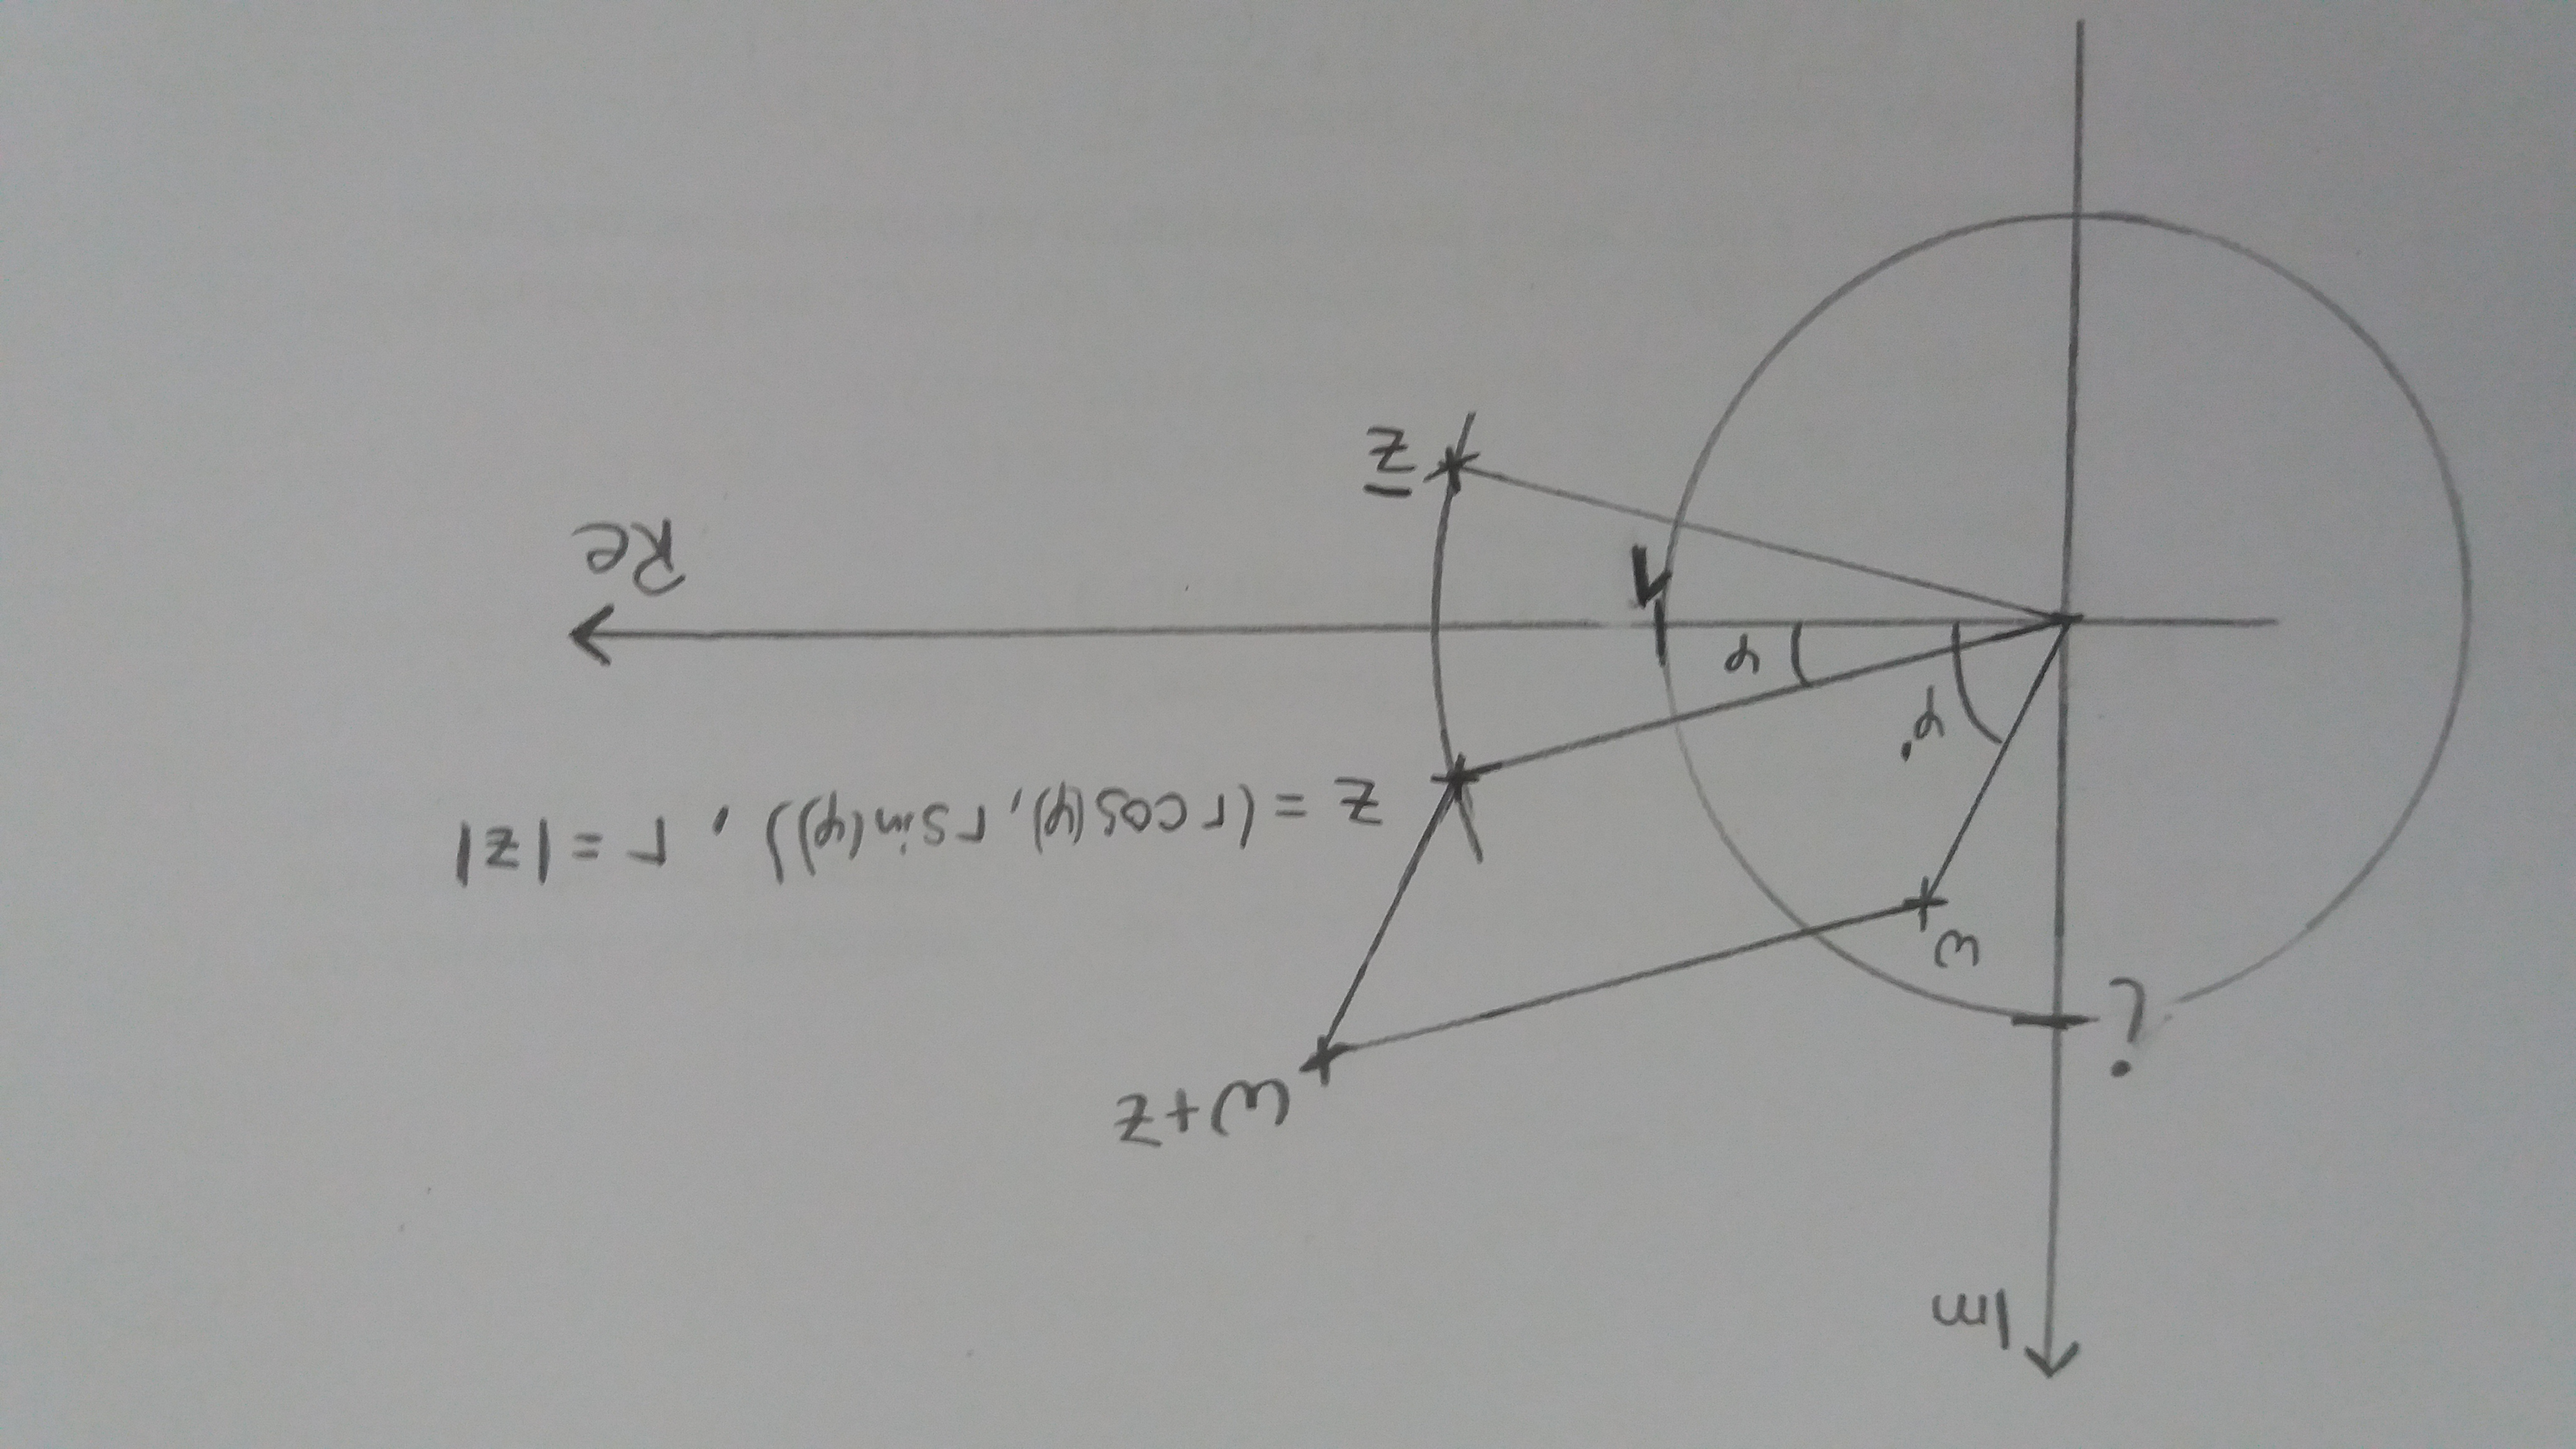
\includegraphics[scale=0.1, angle=180]{pics/Polar.jpg} \\
\end{bemerkung}


\textbf{Proposition: }\\
\begin{eqnarray*}
\mathds{R}^x_+ &=& \{z \in \mathds{C}| x > 0\} \\
\mathds{C}^x &=& \{ z \in \mathds{C} | z \neq 0\} =  \mathds{C} \setminus\{0\} 
\end{eqnarray*}

\begin{itemize}
	\item
	Die Polarkoordinatendarstellungsabbildung:
	\begin{eqnarray*}
	\mathds{R}^x_+ \times \mathds{C} \\
	(r,\varphi) \mapsto z = r(cos(\varphi),i sin(\varphi))
	\end{eqnarray*}
	ist surjektiv.
	\item
	Aus $z = z', d.h.\quad r(cos(\varphi, i sin(vaphi)) = r'(cos(\varphi', i sin(\varphi'))$\\
	...\\$r(cos(\varphi, i sin(\varphi))$
\end{itemize}
\begin{bew}
	Aus reellen Analysis folgt: \\
	jedes $z = (x,y) \neq (0,0)$ kann eindeutig geschrieben werden als $z = (r cos(\varphi), rsin(\varphi))$. \\
	Daher ist r eindeutig bestimmt durch $r = \sqrt{x^2 + y^2}$ \\
	$\varphi$ ist jedoch nur eindeutig bis auf ganzzahlig Vielfache von $2\pi$
\end{bew}


\begin{definition}
	Sei $z \in \mathds{C}$. Jedes $\varphi \in  \mathds{R}$ mit $z =r(cos(\varphi, i sin(\varphi))  $ heißt ein \textbf{Argument von z}. Wir schreiben $\varphi = arg(z)$.
	Falls $\varphi \in (\-\pi,\pi]$ , heißt $\varphi$ \textbf{Hauptwert des Arguments von z}. Wir schreiben $\varphi = Arg(z)$.
\end{definition}

\subsection{Einführung}

\begin{beispiel}
$z = \frac{1}{1+i} = \frac{1}{2} - \frac{i}{2}$\\
$|z| = \frac{1}{\sqrt{2}}, z = \frac{1}{\sqrt{2}}(\cos(-\pi/4)+i\sin(-\pi/4))$
\end{beispiel}

\begin{lemma}
\[
(\cos\phi + i\sin\phi)(\cos\phi\prime + i\sin\phi\prime))
\]
\[ \text{mit anderen Worten } arg(z*z\prime) = arg(z)+ arg(z\prime)
\]
\end{lemma}

\begin{bew}
Additionstheorem der Winkelfkt.
\end{bew}
\begin{bemerkung}
%%%%%%%Lukas Bild 1%%%%%%
\end{bemerkung}

\begin{definition}
$z \in \C $ heißt \textbf{m-te Einheitswurzel}, falls gilt $z^m = 1 \quad, m \in \N$
\end{definition}
\begin{satz}
Zu jedem $m \in \N$ gibt es genau m verschiedene m-te Einheitswurzeln:
\[
\zeta^{(m)}_k := \cos(2\pi\frac{k}{m})+i\sin(2\pi\frac{k}{m})\quad, k=0,\dots,m-1
\]
Beweis Übungsaufgabe 3.
\end{satz}

\subsection{Konvergente Folgen und Reihen}
\begin{definition}
Eine Folge $(z)_{n \in \N}, z_n \in \C$ heißt \textbf{Nullfolge}, falls $\forall \veps > 0 \quad \exists N \in \N$ mit: 
\[|z_n| < \veps \quad ,\forall n>N.\] \\
Eine Folge $(z_n)_{n\in \N}, z_n \in \C$ \textbf{konvergiert gegen z} $\in \C$
falls die Folge $(z_n-z)_{n\in \N}$ ein Nullfolge ist. Der Grenzwert ist eindeutig bestimmt: 
$\begin{displaystyle}
	z = \lim_{n \to \infty}z_n
\end{displaystyle}$
\end{definition}

\begin{bemerkung}
\leavevmode
\begin{itemize}
	\item[1)] Sei $(z_n)_{n\in\N},z_n \in \C$ eine Folge , $z \in \C$.
	\[\lim_{n\to\infty} z_n = z \Leftrightarrow (\lim_{n\to\infty}Re(z_n)=Re(z) \land\lim_{n\to\infty}Im(z_n)=Im(z)) \]
	\item[2)] Sei $(w_n)_{n\in\Z},w_n \in \C$ weitere Folge, mit $w = \lim_{n \to \infty} w_n$
	\begin{eqnarray*}
		&&\lim_{n \to \infty}(z_n \pm w_n) = z \pm w\\
		&&\lim_{n \to \infty}z_nw_n = zw\\
		&&\lim_{n \to \infty}|z_n| = |z| \\
		&&\lim_{n \to \infty}\overline{z}_n = \overline{z} \\
		&&\lim_{n \to \infty} \frac{1}{z_n}= \frac{1}{z}\quad \text{, falls } z_n \neq 0, z\neq 0
	\end{eqnarray*}
\end{itemize}
\end{bemerkung}

\begin{definition}
Sei $(z_n)_{n\in\N}, z_n \in \C$, eine Folge.\\
Die Folge der Partialsummen $(S_n)_{n\geq 0}$ mit $S_n := z_0+\dots+z_n$ heißt die der \textbf{Folge $(z_n)$ zugeordnete Reihe}.
Falls $(S_n)$ konvergiert, so heißt 
$\begin{displaystyle}
	S:=\lim_{n\to \infty} S_n
\end{displaystyle} $ Wert der Reihe und wir schreiben $\begin{displaystyle}
	\sum^\infty_{n=0}z_n := S.
\end{displaystyle}$\\
Eine Reihe 
$\begin{displaystyle}
\sum^\infty_{n=0} z_n
\end{displaystyle}$ heißt \textbf{absolut konvergent} falls die Reihe 
$\begin{displaystyle}
\sum^\infty_{n=0} |z_n|
\end{displaystyle}$ konvergiert.
\end{definition}

\begin{beispiel}
Die geometrische Reihe konvergiert für alle $z \in \C$ zu
$\begin{displaystyle}
	\sum_{\infty}^{n=0} z^n = \frac{1}{1-z}
\end{displaystyle}$
, falls $|z| <  1$ divergiert für $|z| \ge 1$
\end{beispiel}
\begin{bew}
	Es gilt: 
	$\begin{displaystyle}
	\sum_{n=0}^{N} z^n = \frac{1- z^{N+1}}{1-z}\\
	\lim_{n \to \infty} z^n = 0
	\end{displaystyle}$, falls $|z| > 1 \text{ und } |z^n| \ge 1 \text{ falls } |z| \ge 1$
\end{bew}

\begin{satz}
Eine absolut konvergente Reihe konvergiert.
\end{satz}
\begin{bew}
Analysis 1 und Bemerkung 2.2.1
\end{bew}

\begin{definition}
Da die Reihe
\[
\sum^\infty_{n=0} \frac{z^n}{n!}, \sum^\infty_{n=0} \frac{(-1)^n z^{2n}}{(2n)!}, \sum^\infty_{n=0} \frac{(-1)^nz^{2n+1}}{(2n+1)!}
\]
absolut konvergent für alle $z \in \C$ definieren wir: \\
\begin{eqnarray*}
	\exp(z) &=& \sum^\infty_{n=0} \frac{z^n}{n!} \\
	\cos(z) &=& \sum^\infty_{n=0} \frac{(-1)^n z^{2n}}{(2n)!} \\
	\sin(z) &=& \sum^\infty_{n=0} \frac{(-1)^nz^{2n+1}}{(2n+1)!}
\end{eqnarray*}
\end{definition}

\begin{lemma}[Multiplikationssatz von Cauchy]

Seien $\begin{displaystyle}
\sum^\infty_{n=0} z_n \quad ,\sum^\infty_{m=0} w_m
\end{displaystyle}$ absolut konvergente Reihen dann gilt:
\[
(\sum^\infty_{n=0} z_n)(\sum^\infty_{m=0} w_m) = \sum^\infty_{n=0} \sum^n_{k=0} z_k w_{n-k}
\]
und die rechte Seite ist ebenfalls absolut konvergent.
\end{lemma}
\begin{bew}
Kopie des Bew. aus Analysis 1
\end{bew}

\begin{satz}
\[
\exp(z) \exp(w) = \exp(z+w)\quad \forall z,w \in \C
\]
\end{satz}
\begin{bew}
\[
\sum \frac{z^n}{n!} \sum \frac{w^m}{m!} = \sum \sum \frac{z^kw-k}{n!(n-k)!} = \sum \frac{(z+w)^n}{n!}
\]
\end{bew}

\begin{korollar}\label{korollar1}
	\begin{eqnarray*}
		\exp(z) &\neq& 0\\
		\exp(z)^n &=& \exp(nz)\\
		\exp(iz) &=& \cos(z) + i \sin(z)\\
		\cos(z) &=& \frac{1}{2} (\exp(iz)+\exp(-iz))\\
		\sin(z) &=& \frac{1}{2i} (\exp(iz)-\exp(-iz))\\
		\text{sei z = x + iy, } \exp z &=& e^x ( \cos(y) + i \sin(y)) \\
		|\exp(z) | &=& e^x\\
		\cos(z+w) &=& \cos(z)\cos(w) - \sin(z) \sin(w)\\
		\sin(z+w) &=& \cos(z) \sin(w) + \sin(z) \cos(w)
	\end{eqnarray*}
\end{korollar}

\begin{bemerkung}\label{bemerkung1}
$\exp(z)$ ist nicht injektiv, da $\exp(2\pi i k ) = 1 \quad\forall k \in \Z$.\\
Genauer $ \exp(z) = \exp(w) \Leftrightarrow z-w \in 2\pi i \Z$ \\
also $ker( \exp) = \{z \in \C| \exp(z) = 1\} = 2\pi i \Z$ \\
\[\exp( z+w) = \exp( z) \quad\forall z \in \C \Leftrightarrow w \in ker (\exp).\]\\
Die Exponentialfunktion \textbf{ist periodisch} mit Perioden $2 \pi i k, k \in \Z$.\\
\begin{eqnarray*}
	\sin z = 0 &\Leftrightarrow & z = k\pi, k \in \Z \\
	\cos z = 0 &\Leftrightarrow & z = (k+ 1/2)\pi, k \in \Z
\end{eqnarray*}
\end{bemerkung}

Sei
$ S = \{ w \in \C| -\pi < Im(w) \leq \pi\}$\\
$\exp|_S$ ist injektiv, wegen Periodizität
\begin{eqnarray*}
	\{\exp(z)| z \in S\} = \{ \exp(z) | z \in \C\}\\
	\Rightarrow \{ \exp(z) | z \in \C \} = \C^{\times}\\
	\exp|_S: S \to \C^{\times}\\
	z \mapsto \exp (z) \text{ ist bijektiv}
\end{eqnarray*}

\begin{definition}
Wegen Bemerkung \ref{bemerkung1} existiert eine eindeutig bestimmte Zahl $w\in S \text{ mit } \exp(w)= z$. w heißt \textbf{Hauptwert des Logarithmus von z} und wir schreiben $w = Log(z) $
\end{definition}
\begin{satz}
	\leavevmode
\begin{itemize}
	\item[1)]
	Es existiert eine Funktion, der sogenannte \textbf{Hauptzweig des Log}, $ Log: \C^{\times} \to \C$ , welche durch $ \exp(Log(z)) = z \text{ und } -\pi< Im(Log (z)) \leq \pi$ eindeutig bestimmt ist.
	\item[2)]
	$\exp (w) = z \Rightarrow w = Log( z) + 2 \pi i , k \in \Z$
	\item[3)]
	$Log (z) = \log (z)$ falls $ z \in \R^{\times}_+$
	\item[4)]
	$Log (z) = \log(|z|) + i Arg(z)$
\end{itemize}
\end{satz}
\begin{bew}
1) folgt aus Bemerkung \ref{bemerkung1}, ebenso 2) aus 1) und Bem. \ref{bemerkung1}, 3) klar, 4) folgt aus 1),Korollar \ref{korollar1} und ?1.8?
\end{bew}
\subsection{Komplexe Ableitung und Cauchy-Riemannsche Differentialgleichung}
\textbf{Erinnerung:}\\
Eine Funktion $f:D \to \C, D \subset \C$ ist stetig, wenn sie stetig ist aufgefasst als Abb. einer TM $D\subset R^2$ in den $\R^2$.\\
Eine TM $D\subset \R^2$ ist offen, falls zu jedem $q \in D \exists \epsilon > 0: \cup _\epsilon(a) = \{z \in \R^2| |z-a| < \epsilon\} \subset D$.\\
$a \in \C$ ist Häufungspunkt von D, falls $ \forall \epsilon > 0 \exists z \in D$ mit $|z-a| < \epsilon$ .\\

%%%%Lukas f...f schlange...%%%%


\begin{definition}
Eie Funktion $f: D \to \C$ offen, heißt \textbf{komplex differenzierbar in Punkt $a\in D$}, falls:
\[
\lim_{z \to 0} \frac{f(z) -f(a)}{z}-a
\]
existiert. Falls der Grenzwert existiert schreiben wir für den Grenzwert:
\[
f\prime(a) = \frac{df}{dz}(a)
\]
Wenn f in jedem Punkt komplex diffbar ist, dann ist $f\prime$ wieder eine Fkt. auf D.
\end{definition}

\begin{bemerkung}
Alternative Formulierung der komplexen Diffbarkeit:
Die folgenden Aussagen sind äquivalent:
\begin{itemize}
	\item
	1) f ist in $a\in D$ komplex diffbar und hat den Grenzwert l
	\item
	2) $\exists f_1$, stetig in a, mit $f(z) = f_1(z)(z-a), f(a) = l$
	\item
	3) $\exists g: D \to \C$, stetig in a, mit $f(z) = f(a) + (z-a)l+ g(z), g(a)=0$
	\item
	4) $\exists r: D\to \C$, stetig in a, mit $f(z) = f(a) +(z-a)l + r(z), \lim_{z \to a}\frac{r(z)}{z-a}= 0$\\
	Insbesondere folgt: f ist komplex diffbar in a $\Rightarrow$ f stetig in a.
\end{itemize}
\end{bemerkung}

\begin{satz}
Seien $f,g: D \to \C, D\subset \C$, offen, komplex diffbar auf D, Dann sind, f+g, $\lambda$f ($\lambda \in \C$), $f \cdot g, \frac{f}{g}$ ($g(a) \neq 0$) ebenfalls komplex diffbar. Es gelten die üblichen Ableitungsregeln(Ketten-,Produkt-,Quotientenregel).
\end{satz}

\end{document}